\documentclass[a4paper,12pt]{article}

\usepackage[slovene]{babel}
\usepackage[utf8]{inputenc}
\usepackage[T1]{fontenc}
\usepackage{lmodern}

\usepackage{enumitem}
\usepackage{url}
\usepackage{graphicx}
\usepackage{amsthm}

\title{Magicni kvadrati}
\author{Matic Zavadlal}

% https://tex.stackexchange.com/questions/38260/non-italic-text-in-theorems-definitions-examples#38265
\theoremstyle{definition}
\newtheorem{defn}{Definicija}

\theoremstyle{plain}
\newtheorem{thrm}{Izrek}

\newenvironment{dokaz}{%
   \proof[\ttfamily \scshape \large]
   \noindent\textbf{Dokaz.}
   }{
      \endproof
      }

\newcommand{\pojem}[1]{
   \underline{\textsc{#1}}
}

\begin{document}

%%%%%%%%%%%%%%%%%%%%%%%%%%%%%%%%%%%%%%%%%%%%%%%%%%%%%%%%%%%%%%%%%%%%%%%%

\begin{center}
   \LARGE\textbf {Magični kvadrati}
\end{center}


Prirejeno iz virov:
\begin{itemize}[leftmargin=1.6cm]
   \item \url {http://mathworld.wolfram.com/MagicSquare.html}
   \item \url {http://en.wikipedia.org/wiki/Magic_square}
\end{itemize}

\begin{figure}[h]
   \centering
   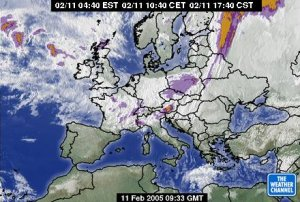
\includegraphics[width=0.5\textwidth]{slika.pdf}
   \label{fig:slika}
\end{figure}

\tableofcontents

%%%%%%%%%%%%%%%%%%%%%%%%%%%%%%%%%%%%%%%%%%%%%%%%%%%%%%%%%%%%%%%%%%%%%%%%

\newpage

%%%%%%%%%%%%%%%%%%%%%%%%%%%%%%%%%%%%%%%%%%%%%%%%%%%%%%%%%%%%%%%%%%%%%%%%

\section{Uvod}


\begin{defn}
   \pojem{Magični kvadrat} reda ?? je nabor ?? različnih števil,
   ki so razvrščena v kvadratno tabelo tako, da vedno dobimo enako vsoto,
   če seštejemo vsa števila poljubne vrstice, vsa števila poljubnega
   stolpca ali vsa števila v katerikoli od glavnih diagonal.
   
   \noindent Primer magičnega kvadrata reda 3 je prikazan v tabeli ??.

   %
   Magični kvadrat reda 3
   %   8 & 1 & 6 \\\hline
   %   3 & 5 & 7 \\\hline
   %   4 & 9 & 2 \\\hline

\end{defn}

\begin{defn}

   Magični kvadrat reda ?? je normalen, če v njem nastopajo števila
   ??

   Magični kvadrat v tabeli ?? je normalen.
   To je tudi najmanjši netrivialni magični kvadrat.
   Poleg normalnih magičnih kvadratov so zanimivi tudi magični kvadrati praštevil.

\end{defn}

%%%%%%%%%%%%%%%%%%%%%%%%%%%%%%%%%%%%%%%%%%%%%%%%%%%%%%%%%%%%%%%%%%%%%%%%

\section{Zgodovina}

\subsection{Kvadrat ">Lo Shu"<}

Kitajska literatura iz časa vsaj 2800 let pred našim štetjem govori o legendi
Lo Shu -- ">zvitek reke Lo"<. V antični Kitajski je prišlo do
silne poplave. Ljudje so skušali rečnemu bogu narasle reke Lo ponuditi daritev,
da bi pomirili njegovo jezo. Iz vode se je prikazala želva z zanimivim vzorcem
na oklepu: v tabeli velikosti tri krat tri so bila predstavljena števila, tako
da je bila vsota števil v katerikoli vrstici, kateremkoli stolpcu in na obeh
glavnih diagonalah enaka: 15. To število je tudi enako številu dni v 24 ciklih
kitajskega sončnega leta. Ta vzorec so na določen način uporabljali upravljalci
reke.

Kvadrat Lo Shu
%   4 & 9 & 2 \\\hline
%   3 & 5 & 7 \\\hline
%   8 & 1 & 6 \\\hline

%%%%%%%%%%%%%%%%%%%%%%%%%%%%%%%%%%%%%%%%%%%%%%%%%%%%%%%%%%%%%%%%%%%%%%%%

\subsection{Kulturna pomembnost}

Magični kvadrati so fascinirali človeštvo skozi vso zgodovino. Najdemo jih
v številnih kulturah, npr.\ v Egiptu in Indiji, vklesane v kamen ali
kovino, uporabljane kot talismane za dolgo življensko dobo in v
izogib boleznim.

\pojem{Kubera-Kolam} je talna poslikava, ki se uporablja v Indiji, in je v
obliki magičnega kvadrata reda 3. Ta je v bistvu enak kot kvadrat
Lo Shu, vendar je vsako število povečano za 19.

Kvadrat Kubera-Kolam
%   23 & 28 & 21 \\\hline
%   22 & 24 & 26 \\\hline
%   27 & 20 & 25 \\\hline

Z magičnimi kvadrati so se ukvarjali tudi najbolj znani matematiki kot na
primer Euler, glej ??.

%%%%%%%%%%%%%%%%%%%%%%%%%%%%%%%%%%%%%%%%%%%%%%%%%%%%%%%%%%%%%%%%%%%%%%%%

\subsection{Zgodnji kvadrati reda 4}

Najzgodnejši znani magični kvadrat reda 4 je bil odkrit na napisu
v Khajurahu v Indiji in v Enciklopediji Bratovščine Čistosti iz enajstega
ali dvanajstega stoletja. Vrh vsega gre celo za ">panmagični kvadrat"<.
V Evropi sta morda najbolj znana naslednja magična kvadrata reda 4:

Magični kvadrat v litografiji Melancholia I (glej sliko ??
za izsek s kvadratom) Albrechta Dürerja naj bi bil najzgodnejši magični kvadrat
v evropski umetnosti. Zelo podoben je kvadratu Yang Huija, ki je nastal na Kitajskem
približno 250 let pred Dürerjevim časom.

Vsoto 34 je mogoče najti pri seštevanju števil v vsaki vrstici, vsakem stolpcu,
na vsaki diagonali, v vsakem od štirih kvadrantov, v sredinskih štirih poljih,
v štirih kotih, v štirih sosedih kotov v smeri urinega kazalca (??), v
štirih sosedih kotov v nasprotni smeri urinega kazalca (??), v dveh naborih
simetričnih parov (?? in ??), in še na nekaj drugih načinov.
Števili na sredini spodnje vrstici tvorita letnico litografije: 1514.

Dürerjev magični kvadrat ??
%   16 &  3 &  2 & 13 \\\hline
%    5 & 10 & 11 &  8 \\\hline
%    9 &  6 &  7 & 12 \\\hline
%    4 & 15 & 14 &  1 \\\hline

Dürerjev magični kvadrat

Pasijonska fasada na katedrali Sagrada família v Barceloni
(glej sliko ?? za fotografijo) vsebuje magični kvadrat reda 4.

Pasijonska fasada, Sagrada Família
%    1 & 14 & 14 &  4 \\\hline
%   11 &  7 &  6 &  9 \\\hline
%    8 & 10 & 10 &  5 \\\hline
%   13 &  2 &  3 & 15 \\\hline

Magični kvadrat na Sagradi Famíliji

Vsota števil v vrsticah, stolpcih oziroma na diagonalah je 33 -- Jezusova starost
v času pasijona. Strukturno je kvadrat podoben Dürerjevemu, vendar so števila
v štirih poljih zmanjšana za 1. Posledica je, da sta števili 10 in 14 podvojeni
in zato kvadrat ni normalen.

%%%%%%%%%%%%%%%%%%%%%%%%%%%%%%%%%%%%%%%%%%%%%%%%%%%%%%%%%%%%%%%%%%%%%%%%

\section{Osnovne lastnosti}

\begin{defn}

   Vsoto ene vrstice, enega stolpca ali ene od glavnih diagonal
   v magičnem kvadratu imenujemo \pojem{magična konstanta}.

\end{defn}

\begin{thrm}

   Magična konstanta normalnega magičnega kvadrata reda ??
   je enaka
   ??

\end{thrm}

\begin{dokaz}
   V normalnem magičnem kvadratu reda $n$ je vsota vseh nastopajočih
   števil (glej ?? na strani ??) enaka
   ??. Ker imamo
   v kvadratu ?? vrstic z enako vsoto, je vsota števil v eni vrstici
   enaka številu ??.
\end{dokaz}

Preprost račun pokaže, da je konstanti ?? analogna konstanta
?? za magični kvadrat, v katerem so nameščena števila
??, ??, ??, ??, ??, enaka
??
Kvadratu v tabeli ?? ustrezata konstanti ?? in ??.

\begin{defn}
   Če vsako od števil v normalnem magičnem kvadratu reda ?? odštejemo
   od števila ??, dobimo nov magični kvadrat, ki je prvotnemu
   \pojem{komplementaren}.
\end{defn}

Na primer, magičnemu kvadratu Lo Shu (glej tabelo ??) priredimo
komplementarni kvadrat, prikazan v tabeli ??.

Kvadratu Lo Shu komplementarni kvadrat
%   6 & 1 & 8 \\\hline
%   7 & 5 & 3 \\\hline
%   2 & 9 & 4 \\\hline

Vidimo, da je dobljeni kvadrat moč dobiti iz kvadrata Lo Shu tudi z zasukom za
180 stopinj okrog središča, kvadrat iz tabele ?? pa je mogoče dobiti
iz kvadrata Lo Shu z zrcaljenjem preko sredinske vodoravne črte.

Število različnih normalnih magičnih kvadratov

   Pravimo, da sta dva magična kvadrata \pojem{različna}, če enega ni mogoče dobiti
   iz drugega s pomočjo zasukov oziroma zrcaljenj.

Števila različnih normalnih magičnih kvadratov se nahajajo v tabeli ??.

   Število različnih normalnih magičnih kvadratov
      točna vrednost približek
      red 1 2 3 4 5 6
      število kvadratov 1 0 1 880 275305224 ??

Vse normalne magične kvadrate reda 4 je oštevilčil Frénicle de Bessy
leta 1693, glej ??, in jih je moč najti v knjigi ??
iz leta 1982. Število normalnih kvadratov reda 5 je izračunal
R. Schroeppel leta 1973 (glej Gardner ??).
Natančno število vseh različnih normalnih magičnih kvadratov reda 6 ni znano.
Avtorja navedenega približka sta Pinn in Wieczerkowski (glej ??), ki
sta za oceno uporabila simulacijo Monte Carlo in metode statistične mehanike.

%%%%%%%%%%%%%%%%%%%%%%%%%%%%%%%%%%%%%%%%%%%%%%%%%%%%%%%%%%%%%%%%%%%%%%%%

\section{Primeri}

V tabelah ??, ?? in ?? so prikazani
magični kvadrati redov 5, 6 in 9.

Magični kvadrat reda 5
%   17 & 24 &  1 &  8 & 15 \\\hline
%   23 &  5 &  7 & 14 & 16 \\\hline
%    4 &  6 & 13 & 20 & 22 \\\hline
%   10 & 12 & 19 & 21 &  3 \\\hline
%   11 & 18 & 25 &  2 &  9 \\\hline

Magični kvadrat reda 6
%    6 & 32 &  3 & 34 & 35 &  1 \\\hline
%    7 & 11 & 27 & 28 &  8 & 30 \\\hline
%   19 & 14 & 16 & 15 & 23 & 24 \\\hline
%   18 & 20 & 22 & 21 & 17 & 13 \\\hline
%   25 & 29 & 10 &  9 & 26 & 12 \\\hline
%   36 &  5 & 33 &  4 &  2 & 31 \\\hline

Magični kvadrat reda 9
%   47 & 58 & 69 & 80 &  1 & 12 & 23 & 34 & 45 \\\hline
%   57 & 68 & 79 &  9 & 11 & 22 & 33 & 44 & 46 \\\hline
%   67 & 78 &  8 & 10 & 21 & 32 & 43 & 54 & 56 \\\hline
%   77 &  7 & 18 & 20 & 31 & 42 & 53 & 55 & 66 \\\hline
%    6 & 17 & 19 & 30 & 41 & 52 & 63 & 65 & 76 \\\hline
%   16 & 27 & 29 & 40 & 51 & 62 & 64 & 75 &  5 \\\hline
%   26 & 28 & 39 & 50 & 61 & 72 & 74 &  4 & 15 \\\hline
%   36 & 38 & 49 & 60 & 71 & 73 &  3 & 14 & 25 \\\hline
%   37 & 48 & 59 & 70 & 81 &  2 & 13 & 24 & 35 \\\hline

%%%%%%%%%%%%%%%%%%%%%%%%%%%%%%%%%%%%%%%%%%%%%%%%%%%%%%%%%%%%%%%%%%%%%%%%

%%%%%%%%%%%%%%%%%%%%%%%%%%%%%%%%%%%%%%%%%%%%%%%%%%%%%%%%%%%%%%%%%%%%%%%%

\end{document}
